\documentclass[final]{beamer}
\usepackage[size=custom,width=70.7,height=100,scale=1.0]{beamerposter}

\usepackage[brazilian]{babel}
\usepackage[utf8]{inputenc}
\usepackage[T1]{fontenc}

\usepackage{tikz}
\usetikzlibrary{matrix,shapes,positioning,shadows,trees,patterns}

\usepackage[shortlabels]{enumitem}
\usepackage[numbers]{natbib}
\usepackage{subcaption}
\usepackage{pifont}
\bibliographystyle{plainnat}

\sloppy

%----------------------------------------------------------------------------------------
%	SHORTCUTS
%----------------------------------------------------------------------------------------
\newcommand{\B}[1]{\mathbb{#1}}
\newcommand{\Cl}[1]{\ensuremath{\mathcal{#1}}}

\newcommand{\sse}{\Leftrightarrow}
\newcommand{\so}{\Rightarrow}
\newcommand{\se}{\Leftarrow}
\newcommand{\rec}{\leftarrow}

\newcommand{\tdots}{\,.\,.\,}

%----------------------------------------------------------------------------------------
%	BEAMER STYLE
%----------------------------------------------------------------------------------------

\usetheme{poster-exemplo}
\setbeamercolor{block title}{fg=dblue,bg=white}
\setbeamercolor{block body}{fg=black,bg=white}
\setbeamercolor{block alerted title}{fg=dblue,bg=gray!50}
\setbeamercolor{block alerted body}{fg=black,bg=gray!20}
\setbeamercolor{block prob}{fg=black,bg=white}
\setbeamertemplate{caption}[numbered]

%----------------------------------------------------------------------------------------
%	CUSTOM STYLING
%----------------------------------------------------------------------------------------

\newenvironment<>{prob}{
    \begin{beamercolorbox}[sep=1ex,center,dp={1ex}]{block prob}
    \textcolor{dblue}{\textbf{Problema:}}\itshape
\end{beamercolorbox}}

%----------------------------------------------------------------------------------------
%	POSTER
%----------------------------------------------------------------------------------------

\title{Promovendo o Engajamento Estudantil na Universidade (USP-Eventos)}
\author{Bruno Mazetti Saito \hspace{50pt} Willian Hiroshi Takihi \hspace{100pt} Orientador: Flávio Soares Correa da Silva}
\institute{\vspace{10pt}Departamento de Ciência da Computação,
Instituto de Matemática e Estatística, Universidade de São Paulo}


\begin{document}
\begin{frame}[t]
\begin{columns}[t]

\begin{column}{0.48\paperwidth}
    \begin{block}{Motivações e proposta}

        Em uma universidade como a USP, existem várias atividades e eventos que ocorrem diariamente, mas às vezes elas acabam passando despercebidas ou não há um modo fácil de filtrar aquelas que gostaríamos de participar.

        Portanto, a proposta é criar um sistema capaz de compilar eventos universitários publicados em redes sociais, e mostrá-los em uma plataforma acessível aos alunos. Além de criar uma experiência personalizada ao usuário, permitindo que ele indique páginas fonte de seu interesse onde os eventos serão buscados.
    
        \vskip2ex
    \end{block}

    \begin{block}{Demonstração}
        Acesse a plataforma pelo \textit{link} \url{https://uspevents.ix.tc/}.

        \begin{alertblock}{Página principal}
            \begin{figure}[h]
                \centering
                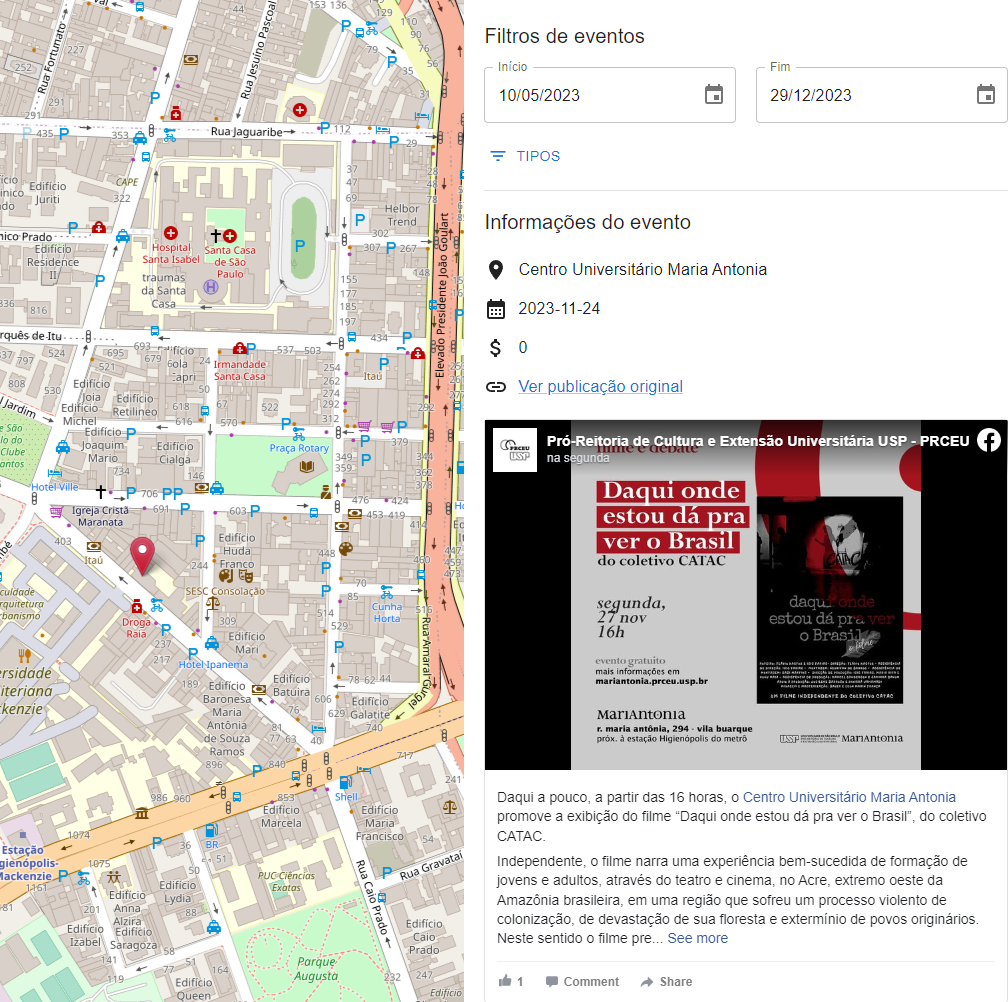
\includegraphics[width=0.95\textwidth]{figuras/paginaInicial.png}
                \caption{Página principal do sistema}
            \end{figure}
        \end{alertblock}
        

        \begin{alertblock}{Filtros e cadastro de usuário}
            \begin{figure}
                \centering
                \begin{minipage}{0.55\textwidth}
                    \centering
                    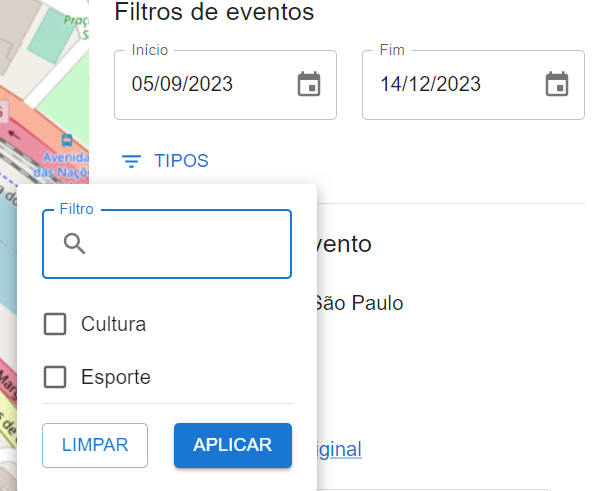
\includegraphics[width=\textwidth]{figuras/filtroEventos.png}
                    \caption{Filtros de eventos}
                \end{minipage}

                \vspace{1cm}
                
                \subfloat[][]{
                    \begin{minipage}{0.40\textwidth}
                        \centering
                        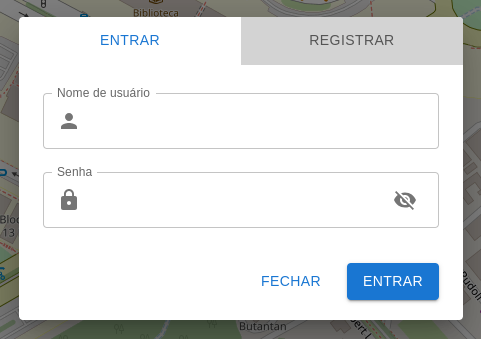
\includegraphics[width=\textwidth]{figuras/loginModal.png}
                    \end{minipage}
                }
                \subfloat[][]{
                    \begin{minipage}{0.40\textwidth}
                        \centering
                        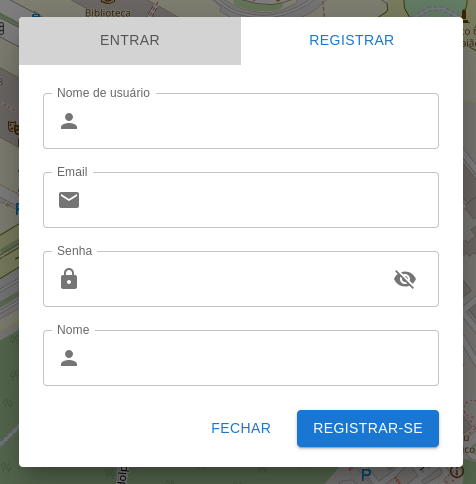
\includegraphics[width=\textwidth]{figuras/registrationModal.png}
                    \end{minipage}
                }
                \caption{(a) \textit{login} e (b) cadastro de usuários}

            \end{figure}
        \end{alertblock}
    \end{block}
\end{column}

\begin{column}{0.48\paperwidth}

    \begin{alertblock}{Registro de \textit{Webpages}}
        \begin{figure}
            \centering
            \begin{minipage}{1\textwidth}
                \centering
                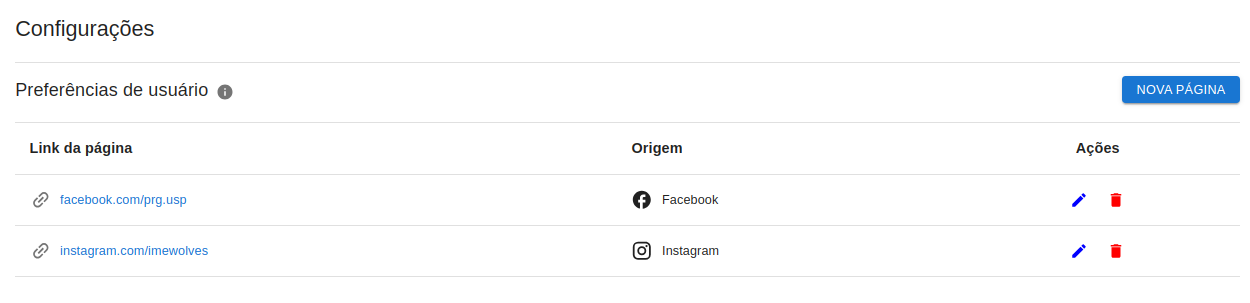
\includegraphics[width=1\textwidth]{figuras/webpagesTable.png}
                \caption{\textit{Webpages} cadastradas}
            \end{minipage}
        \end{figure}
    \end{alertblock}

    \vskip2ex

    \begin{block}{Visão técnica}
        \begin{figure}[h]
            \centering
            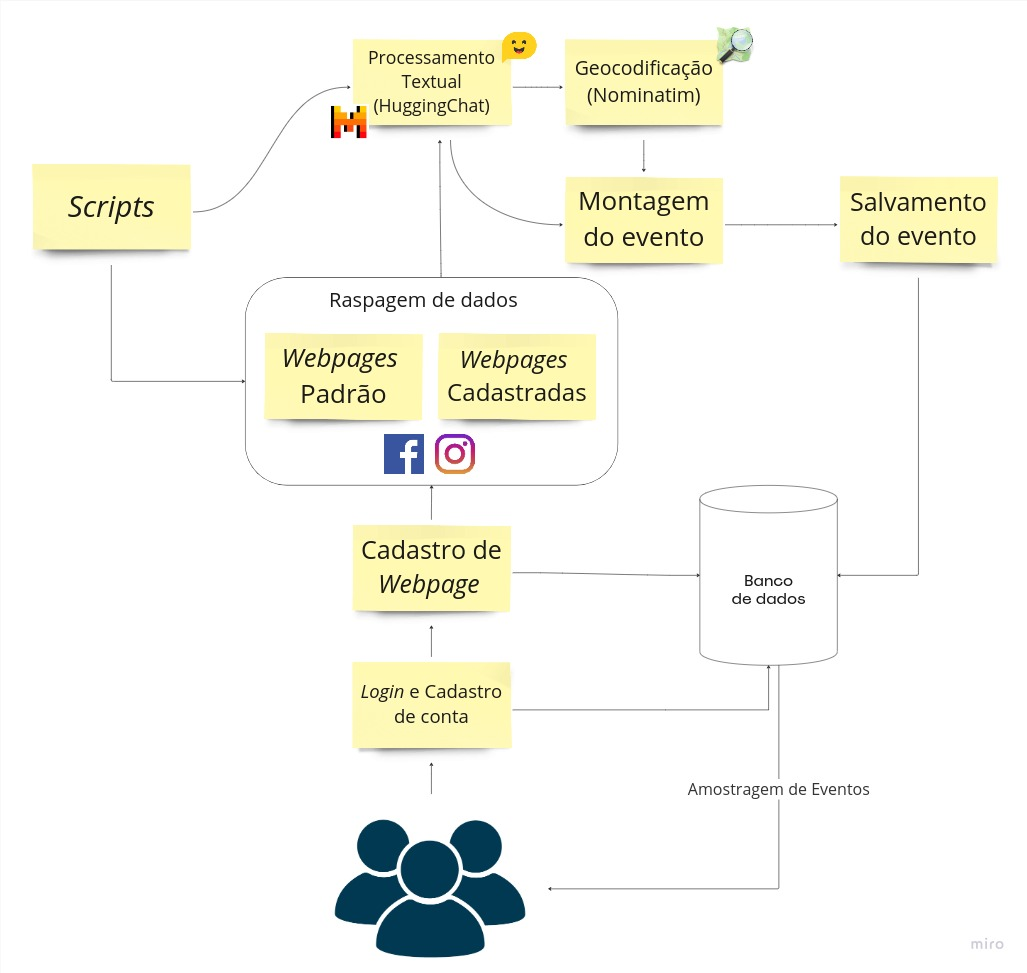
\includegraphics[width=1\textwidth]{figuras/systemDiagram.jpg}
            \caption{Fluxo de funcionamento da plataforma}
        \end{figure}
        
        \vspace{1cm}
        
        \begin{figure}[h]
            \centering
            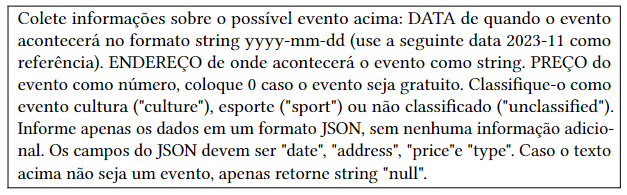
\includegraphics[width=1\textwidth]{figuras/instrucao.png}
            \caption{Instruções para extração de informações de evento}
        \end{figure}
    \end{block}

    \begin{block}{Desafios e Problemas}

        \begin{enumerate}[label=\textbf{\arabic*.}, itemsep=1em]
            \item \textbf{Raspagem de dados}
                \vspace{0.3em}
                \begin{itemize}[label=\ding{113}, itemsep=0.3em]
                    \item Suspensão temporária de acesso às redes sociais
                    \item Imprevisibilidade da estrutura das \textit{webpages}
                \end{itemize}

            \item \textbf{Processamento textual}
                \vspace{0.3em}
                \begin{itemize}[label=\ding{113}, itemsep=0.3em]
                    \item Processo altamente custoso e demorado
                    \item Escolha do modelo de IA generativa
                    \item Estruturar instrução para extração de informações
                \end{itemize}

            \item \textbf{Código aberto}
                \vspace{0.3em}
                \begin{itemize}[label=\ding{113}, itemsep=0.3em]
                    \item Geocodificação: Google Maps vs. Nominatim
                \end{itemize}
        \end{enumerate}

        \vskip2ex
    \end{block}

    \begin{block}{Mais informações}
        Código disponível em: \url{https://github.com/willhiroshi/TCC-USP-Events}
        
        Monografia e mais informações: \url{https://linux.ime.usp.br/~willhiro/mac0499/}
    \end{block}

\end{column}

\end{columns}
% ---------------------------------------------------------------------------- %
\end{frame}
\end{document}
